\chapter{热历史、最后散射与原始汤}

\lectureoverview{宇宙的膨胀历史同时也是一部热历史。我们首先通过平衡来定义温度，又通过散射来定义平衡。光子气体在自由电荷的作用下保持热化，从而获得普朗克谱；当电子与质子结合时，辐射退耦，但随着每一个波长都随尺度因子拉伸，辐射仍保持其黑体形状。光子与物质之间巨大的数量比，进而解释了为什么复合发生在远低于氢电离温度之时。继续向前回溯，我们会依次经过最后散射、物质--辐射相等、电子--正电子对平衡，最终到达湮灭之后残留下来的那一点微小的物质--反物质过剩。}

\section{从模型拟合到热历史}

一个宇宙学模型至少由尺度因子历史和空间几何来指定，
\begin{equation}
a(t),
\qquad
k\in\{+1,0,-1\}.
\end{equation}
实用的方法是：选定模型，计算它预言什么，将这些预言与数据比较，然后调整参数。直接从数据反向进行推断是可能的，但往往不够透明。

从相对较近的源来确定曲率是困难的。正如地球的曲率在短的地面基线上只是一个小修正，当宇宙学基线不够大时，空间曲率也只是一种微弱的效应。这既是缺点也是优点：普通的源巡天不能锐利地确定\(k\)，但\(k\)具有中等程度的不确定性并不妨碍对膨胀历史作出有用的重构。

有两类观测量承担了大部分任务。标准烛光给出亮度随红移的变化，而源巡天给出红移区间内的天体数目。由此得到的拟合倾向于一种包含可观真空能贡献的膨胀历史。要获得精确的曲率信息，则需要宇宙微波背景所提供的长得多的几何力臂。

现在我们改变问题。我们不再只问\(a(t)\)如何演化，而是问宇宙的温度如何演化。这个问题始于一个更基本的问题：在什么条件下，一个系统才具有温度？

\section{宇宙何时具有温度}

温度是热平衡的一种属性。粒子集合通过碰撞趋近平衡，而这些碰撞必须比宏观环境的变化进行得更快。在膨胀宇宙中，有用的比较是
\begin{equation}
\tau_{\rm scatt}\ll H^{-1},
\label{eq:c07-equilibrium-condition}
\end{equation}
其中\(\tau_{\rm scatt}\)是特征散射时间，\(H^{-1}\)是膨胀时间。当这个不等式不成立时，宇宙在碰撞能够恢复平衡之前就已经发生了变化。

考虑一个完全反射的盒子。向其中射入一束激光脉冲，封闭开口，并假设盒中只有光子。脉冲会无限地来回反弹，但普通的低能光子彼此之间的散射极其微弱。仅靠反射并不能把它们的能量重新分配成热谱。因此，光子气体并不会仅仅因为被限制住就实现热化。

自由带电粒子改变了这一情形。电磁波使电子加速；被加速的电荷会再辐射，因此光子能够高效地散射。只要有足够多的自由电子和质子，反复的散射就会在三种粒子之间重新分配能量，直到它们形成一锅具有共同温度的热汤。

在大尺度上，宇宙是电中性的。在最简单的记账中，
\begin{equation}
n_{e^-}=n_p,
\label{eq:c07-neutrality}
\end{equation}
因为电子和质子的电荷大小相等、符号相反。这个方程陈述的是电中性；它并不解释电荷为何是中性的，也不解释为什么两种电荷的大小一致。那些是关于粒子物理的更深层事实。

等离子体与中性气体之间的区别是决定性的。自由电子能高效地散射辐射。一旦电子与质子结合形成中性氢，主导的电场在长距离上相互抵消，散射就变得远不那么有效。在当今宇宙的低密度下，中性物质无法在一个宇宙寿命内使背景光子达到平衡。

在足够高的温度下，高能碰撞反复电离氢，并维持着数量可观的自由电荷。此时电子、质子和光子共享同一个温度。随着系统冷却，原子得以存留，自由电子密度骤降，共同的平衡随之丧失。此后分别赋予物质和辐射的温度不必彼此一致。

\begin{classroomqa}
\audiencequestion{如果微波背景的温度接近\(3\,\mathrm{K}\)，那么这就是今天整个宇宙的温度吗？}
\lecturerresponse{不是。光子谱可以用黑体温度来标记，但当前物质并不与那些光子处于平衡。不同组分具有不同的动理学温度或有效温度，因此今天不存在单一的全局热力学温度。}
\end{classroomqa}

\section{热辐射与量子转折}

平衡辐射场包含由下式联系的各种波长与频率的谱：
\begin{equation}
\nu\lambda=c.
\end{equation}
为避免将辐射亮度与能量密度混淆，令\(u_\nu(T)\)表示单位体积、单位频率的能量：
\begin{equation}
dE=u_\nu(T)\,dV\,d\nu.
\label{eq:c07-spectral-density}
\end{equation}
因此\(u_\nu\)的量纲为能量除以体积和频率。

温度本身就是一个能量标度。历史上的温度单位掩盖了这一事实，因此玻尔兹曼常数提供了换算：
\begin{equation}
E_{\rm thermal}\sim k_B T.
\end{equation}
在自然单位制中可以令\(k_B=1\)，但保留它能使开尔文与能量保持可见的区别。

在量子力学之前，利用\(k_BT\)、\(\nu\)和\(c\)进行量纲分析，得到瑞利--金斯谱能量密度，
\begin{equation}
u_\nu^{\rm RJ}(T)=\frac{8\pi\nu^2}{c^3}k_BT.
\label{eq:c07-rayleigh-jeans}
\end{equation}
数值因子取决于对电磁模式的计数，但本质的经典行为是\(u_\nu\propto T\nu^2\)。它随频率增加而无限制地上升，因此预言
\begin{equation}
\int_0^\infty u_\nu^{\rm RJ}\,d\nu=\infty.
\end{equation}
这个不可能的结果就是紫外灾难。而实测谱则先上升、随后转折，并下降得足够快，从而包含有限的能量。

普朗克常数引入了缺失的量子标度。对于方程~\eqref{eq:c07-spectral-density}中定义的谱能量密度，普朗克定律为
\begin{equation}
u_\nu(T)
=
\frac{8\pi h\nu^3}{c^3}
\frac{1}{e^{h\nu/(k_BT)}-1}.
\label{eq:c07-planck}
\end{equation}
指数依赖于无量纲比值
\begin{equation}
x=\frac{h\nu}{k_BT},
\end{equation}
因为\(E_\gamma=h\nu\)和\(k_BT\)都是能量。

在低频下，\(x\ll1\)，并且
\begin{equation}
e^x-1=x+O(x^2).
\end{equation}
代入方程~\eqref{eq:c07-planck}得到
\begin{align}
u_\nu(T)
&\simeq
\frac{8\pi h\nu^3}{c^3}
\frac{k_BT}{h\nu}
\\
&=
\frac{8\pi\nu^2}{c^3}k_BT,
\end{align}
因此经典物理在其适当的低频范围内得到恢复。在高频下，\(x\gg1\)，指数项占主导并压制了谱。转折发生在
\begin{equation}
\frac{h\nu}{k_BT}\sim1.
\label{eq:c07-crossover}
\end{equation}
这就是量子转折取代经典上升的点。

\begin{figure}[htbp]
\centering
\includegraphics[width=0.82\textwidth]{lecture_07_figure_02.png}
\caption{黑板上的热转折。裁剪后的上方表达式是\(h\nu/(kT)>1\)，清晰可见的下方表达式是\(hc/(kT)>\lambda\)。下方黑板上模糊的残留不作为方程证据使用。}
\label{fig:c07-thermal-board}
\lectureframe{00:44:42.840}
\end{figure}

利用\(\nu=c/\lambda\)，转折定义了一个数量级的热波长，
\begin{equation}
\boxed{\lambda_{\rm th}\sim\frac{hc}{k_BT}}.
\label{eq:c07-thermal-wavelength}
\end{equation}
更短的波长位于指数压制的尾部；大部分功率由这一数量级的波长携带，具体数值因子取决于谱是按单位频率还是按单位波长绘制的。

\begin{classroomqa}
\audiencequestion{普朗克是从这里使用的电子--质子等离子体模型得到该谱的吗？}
\lecturerresponse{不是。他将经验谱信息与维恩位移定律结合起来，后者已经表明峰值波长与温度成反比变化。这种标度关系揭示了一个新的常数\(h\)。普朗克将结果与材料壁中的振子联系起来，而对辐射场的完整量子解释则是后来才出现的。\lecturetimestamp{00:37:06--00:39:25}}
\end{classroomqa}

\begin{classroomqa}
\audiencequestion{为什么量纲检验似乎漏掉了一个\(c\)的幂次？}
\lecturerresponse{最初被称为强度的量被定义为每体积每频率的能量，而含有\(2h\nu^3/c^2\)的熟悉公式是每面积每立体角的谱辐射亮度。谱能量密度带有\(c^{-3}\)和一个角度因子，如方程~\eqref{eq:c07-planck}所示。这一修正改变的是归一化约定，而不是无量纲比值\(h\nu/(k_BT)\)或热波长。\lecturetimestamp{00:39:33--00:44:51}}
\end{classroomqa}

除归一化之外，普朗克谱具有普适的形状。方程~\eqref{eq:c07-planck}可以写成
\begin{equation}
u_\nu(T)=T^3\,F\!\left(\frac{\nu}{T}\right),
\label{eq:c07-scaling-form}
\end{equation}
其中常数被吸收进\(F\)。提高\(T\)会重新标度频率轴和整体高度；同一条无量纲曲线会再次出现。用波长语言来说，提高温度会将谱向更短的波长压缩。

\begin{figure}[htbp]
\centering
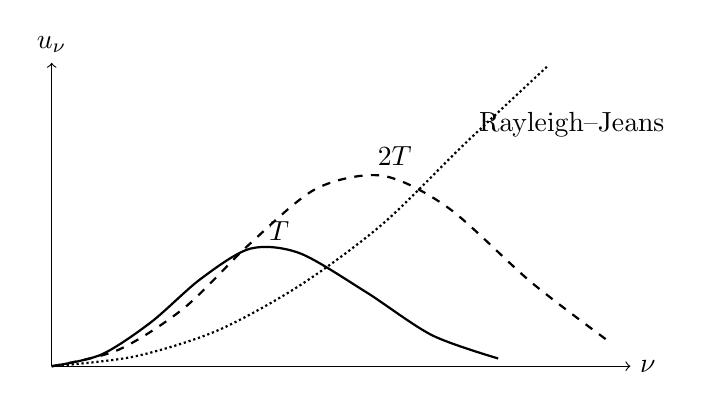
\begin{tikzpicture}[x=1.05cm,y=0.82cm]
\draw[->] (0,0)--(7.0,0) node[right] {\(\nu\)};
\draw[->] (0,0)--(0,4.7) node[above] {\(u_\nu\)};
\draw[densely dotted,thick] plot[smooth] coordinates
  {(0,0) (1,0.15) (2,0.55) (3,1.25) (4,2.20) (5,3.45) (6,4.65)};
\draw[thick] plot[smooth] coordinates
  {(0,0) (0.6,0.18) (1.2,0.68) (1.8,1.35) (2.4,1.82) (3.0,1.75) (3.8,1.15) (4.6,0.48) (5.4,0.12)};
\draw[thick,dashed] plot[smooth] coordinates
  {(0,0) (0.8,0.25) (1.6,0.90) (2.4,1.90) (3.2,2.75) (4.0,2.95) (4.8,2.45) (5.8,1.30) (6.7,0.42)};
\node[anchor=west] at (5.05,3.75) {Rayleigh--Jeans};
\node at (2.75,2.10) {\(T\)};
\node at (4.15,3.25) {\(2T\)};
\end{tikzpicture}
\caption{经典谱无限制地上升，而普朗克谱则发生转折。提高温度会将特征频率向上移动，并保持无量纲形状不变。}
\label{fig:c07-planck-redraw}
\end{figure}

当今宇宙中的绝大多数光子属于微波背景，其特征波长约为毫米量级。方程~\eqref{eq:c07-thermal-wavelength}将该波长与几开尔文联系起来，此处按惯例取整为\(3\,\mathrm{K}\)。仅凭波长只能给出粗略的关联。更强的证据是，在众多频率上进行的测量以极高精度描绘出了完整的黑体曲线。

\begin{classroomqa}
\audiencequestion{一个微波背景光子占据多大空间？}
\lecturerresponse{光子没有普遍存在的、边界分明的尺寸。它可以被制备成波包，其空间延展取决于所处状态，而它的波长则设定了其振荡的尺度。对于热背景而言，特征波长和自然的波包尺度都在毫米量级，但两者都不应被误认为某个经典小物体的半径。\lecturetimestamp{00:57:16--00:59:05}}
\end{classroomqa}

\section{膨胀冻结了黑体形状}

从一个包含电离氢和处于平衡态的辐射的热盒子开始。随着盒子膨胀，其内容物做功，能量密度下降，温度降低。最终电子和质子保持束缚成为中性原子。原子的形成被称为\emph{复合}；有效光子--物质散射的丧失被称为\emph{退耦}。这两个过程密切相关，但命名的是不同的物理事件。

退耦之后，物质和辐射不再共享同一温度。然而光子谱仍保持其普朗克形式。每一个自由传播的波长都被同一膨胀因子拉伸，
\begin{equation}
\lambda\propto a,
\qquad
\nu\propto a^{-1}.
\end{equation}
由于普朗克曲线依赖于\(\nu/T\)，这种均匀红移等价于给辐射指定一个温度
\begin{equation}
\boxed{T_\gamma\propto a^{-1}.}
\label{eq:c07-temperature-scaling}
\end{equation}
因此，即使没有碰撞不断重建，膨胀仍保持其形状。物质则遵循其自身后来的热历史。

因此，观测到的微波背景是一种化石平衡分布。它的黑体形式是在自由电荷高效散射的时期建立起来的，随后由均匀的宇宙学红移携带至今。星光、伽马射线以及其他后来的源确实存在，但它们在数量上远小于遗迹光子群体，并且具有可辨认的天体物理起源。

\begin{classroomqa}
\audiencequestion{辐射在不再与物质处于平衡态之后，如何仍能保持黑体谱？}
\lecturerresponse{碰撞是产生平衡谱所必需的，但在完全均匀的膨胀下，碰撞并非保持平衡谱所必需。将每一个波长乘以同一因子，就把一个普朗克谱映射为另一个温度更低的普朗克谱。光子不再与物质共享温度，但保留着它们自己的黑体温度。}
\end{classroomqa}

\section{为什么复合发生得如此之晚}

今天的波长与退耦时的波长之间的关系为
\begin{equation}
\frac{\lambda_0}{\lambda_{\rm dec}}
=
\frac{a_0}{a_{\rm dec}}
=
\frac{T_{\rm dec}}{T_0}.
\label{eq:c07-decoupling-ratio}
\end{equation}
退耦在数学上并非瞬时发生，但与随后的历史相比足够短暂，因此可以给它指定一个特征标度因子和温度。此处\(T_0\)指的是CMB温度，而非星系际物质的动理学温度。

氢的基态电离能为
\begin{equation}
\chi_H=13.6\,\mathrm{eV}.
\end{equation}
初步猜测会令\(k_BT\sim\chi_H\)，从而一个典型光子就能电离一个原子。这个猜测实在太高了，因为热谱包含高能尾部，而且宇宙包含数量巨大的光子。

\begin{figure}[htbp]
\centering
\includegraphics[width=0.82\textwidth]{lecture_07_figure_03.png}
\caption{黑板上引入了观测到的丰度比\(N_\gamma/N_e=10^8\)和光子能量符号\(\epsilon\)。图中只能看到指数项的起始部分；完整的玻尔兹曼因子由口头推导得出。}
\label{fig:c07-boltzmann-board}
\lectureframe{01:06:10.631}
\end{figure}

此处使用的取整丰度比为
\begin{equation}
\frac{N_\gamma}{N_e}\sim10^8.
\label{eq:c07-photon-electron-ratio}
\end{equation}
它是通过将测得的CMB光子密度与普通物质清单进行比较而推断出来的。对于光子能量\(\epsilon\)，高能尾部具有玻尔兹曼形式
\begin{equation}
P(\epsilon)\propto e^{-\epsilon/(k_BT)}.
\end{equation}
因此，每个原子可获得的电离光子数估计为
\begin{equation}
10^8 e^{-\chi_H/(k_BT)}.
\end{equation}
直到该量降至量级为1之前，电离一直有效。

取对数得到
\begin{equation}
\frac{\chi_H}{k_BT}
\sim
\ln 10^8
\simeq18.4,
\end{equation}
或者，按所需的精度，
\begin{equation}
k_BT\sim\frac{\chi_H}{20}.
\label{eq:c07-tail-estimate}
\end{equation}
特征光子可以远低于阈值，因为对每个原子而言，来自尾部的哪怕一个电离光子就足够了。

\begin{classroomqa}
\audiencequestion{尾部估计是恰好计入阈值处的光子，还是计入阈值以上的所有光子？}
\lecturerresponse{它计入阈值处及以上的光子。由于尾部按指数衰减，该积分的大部分来自能量接近\(\chi_H\)的光子，因此简单的指数估计就能抓住相关的数量级。\lecturetimestamp{01:08:39--01:08:54}}
\end{classroomqa}

\begin{classroomqa}
\audiencequestion{在解耦时，比值\(N_\gamma/N_e\)是否也约为\(10^8\)？}
\lecturerresponse{在此处所用的近似下，是的。从解耦回溯到温度高得多的时期，膨胀以相同的体积因子稀释这两个粒子群，并且没有产生或消灭足够多的任一粒子种类来改变它们的比值。在更高的温度下，对产生反应需要新的记账。\lecturetimestamp{01:08:54--01:09:57}}
\end{classroomqa}

\begin{classroomqa}
\audiencequestion{恒星发出的光子对这一计数有可观贡献吗？}
\lecturerresponse{没有。在复合时期恒星尚不存在，而且即使在今天，它们的光子也只是宇宙微波背景粒子群中极小的一部分。式~\eqref{eq:c07-photon-electron-ratio}中的比值涉及的是遗留的热光子。\lecturetimestamp{01:11:44--01:12:39}}
\end{classroomqa}

\begin{classroomqa}
\audiencequestion{当电子与质子复合时，发射出的光子是否应在黑体谱中留下一个尖锐的氢特征？}
\lecturerresponse{只要散射和吸收与膨胀相比仍然足够快，辐射就会被不断重新处理，并保持接近热平衡。足够突然的冻结可以保留一种畸变，但缓慢的、接近平衡的复合阻止了一条大的孤立谱线取代黑体形式。\lecturetimestamp{01:12:42--01:14:07}}
\end{classroomqa}

由此得到的课堂估计为\(T_{\rm dec}\sim4\times10^3\,\mathrm{K}\)。对\(\chi_H/20\)作直接换算会给出略高一些的数值，从而提示有效分母可能更接近\(40\)。这并不矛盾；它暴露出用一个尾部计数代替完整电离平衡的粗糙性。受控的平衡处理使用萨哈关系，
\begin{equation}
\frac{x_e^2}{1-x_e}
=
\frac{1}{n_H}
\left(\frac{m_e k_BT}{2\pi\hbar^2}\right)^{3/2}
e^{-\chi_H/(k_BT)},
\label{eq:c07-saha}
\end{equation}
随后是非平衡复合动力学。这个粗略论证之所以有价值，是因为它指出了主导物理：极小的重子与光子之比把中性原子的存活推迟到远低于\(\chi_H/k_B\)的温度。

\section{红移到最后散射面}

取\(T_0\simeq3\,\mathrm{K}\)和\(T_{\rm dec}\sim4\times10^3\,\mathrm{K}\)，式~\eqref{eq:c07-decoupling-ratio}给出
\begin{equation}
\boxed{
\frac{a_0}{a_{\rm dec}}
\sim
\frac{T_{\rm dec}}{T_0}
\sim10^3
}.
\label{eq:c07-decoupling-expansion}
\end{equation}
等价地，最后散射红移约为\(10^3\)量级。在这一时期之前，电离等离子体是不透明的；在此之后，光子几乎自由地传播。

这一热事件发生在热膨胀开始之后仅几十万年，按交流中的习惯说法约为\(380{,}000\)年。与随后的宇宙年龄相比，这一间隔微不足道。自解耦以来，长度增长了约\(10^3\)倍，共动体积元增长了约\(10^9\)倍。

解耦是一个热标志，而不是这中间历史中唯一的事件。星系形成、恒星形成和黑洞形成都发生得更晚，但这里将它们搁置一旁，以便干净地回溯热标志。

向外看就是向过去看。近处的壳层显示较近的时期；更远处的壳层显示更早的时期。我们的过去光锥最终与复合时期相遇，而它与该时期的交集就是最后散射面。更早的电磁辐射被自由电荷反复散射，无法直接到达我们这里。

\begin{figure}[htbp]
\centering
\begin{coursefitfigure}
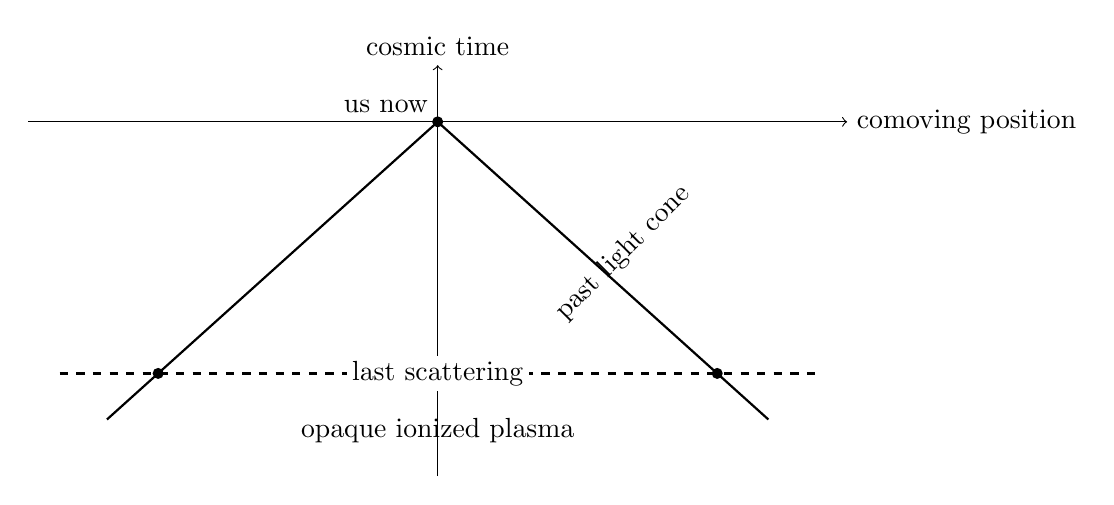
\begin{tikzpicture}[x=1.0cm,y=0.9cm]
\draw[->] (0,0)--(0,5.8) node[above] {cosmic time};
\draw[->] (-5.2,5.0)--(5.2,5.0) node[right] {comoving position};
\draw[thick] (0,5.0)--(-4.2,0.8);
\draw[thick] (0,5.0)--(4.2,0.8);
\draw[thick,dashed] (-4.8,1.45)--(4.8,1.45);
\fill (0,5.0) circle (2pt) node[above left] {us now};
\fill (-3.55,1.45) circle (2pt);
\fill (3.55,1.45) circle (2pt);
\node[fill=white,inner sep=2pt] at (0,1.45) {last scattering};
\node at (0,0.65) {opaque ionized plasma};
\node[rotate=45] at (2.35,3.15) {past light cone};
\end{tikzpicture}
\end{coursefitfigure}
\caption{电磁观测沿着过去光锥回溯，只能到达最后散射面。更早的光子被电离等离子体反复散射。}
\label{fig:c07-last-scattering}
\end{figure}

\begin{classroomqa}
\audiencequestion{解耦是否终结了对更早时期的一切可能观测？}
\lecturerresponse{它终结了直接的电磁观测，因为等离子体对光子是不透明的。相互作用更弱的信使可以更早逃逸：遗留中微子在原则上探测更深的一层，而引力辐射可以携带来自更早时期的信息。因此，我们在最后散射之外的大部分知识是间接的，但并非任意的。\lecturetimestamp{01:32:27--01:36:31}}
\end{classroomqa}

\begin{classroomqa}
\audiencequestion{\(a\)在开始时绝对值为多少，宇宙是否必然是一个微小的有限物体？}
\lecturerresponse{在平坦空间中，只有标度因子之比具有不变意义；\(a\)的归一化是任意的。负曲率空间切片也可以是无限的。闭合的\(k=+1\)宇宙具有有限的曲率半径，但观测仍然确定的是膨胀比，而不是已知的原始大小。热大爆炸本身并不等于说全部空间曾是一个微小球体。\lecturetimestamp{01:30:05--01:32:22}}
\end{classroomqa}

\begin{classroomqa}
\audiencequestion{由于CMB比星系更古老，看到它是否能告诉我们今天在我们可观测区域之外是否存在星系？}
\lecturerresponse{不能。CMB显示的是遥远区域在解耦时的样子，而不是它今天的样子。来自足够遥远距离的当今星系的光还没有时间到达我们这里。支持我们视界之外仍有星系持续存在的是观测到的大尺度均匀性以及没有可见边缘，而不是CMB提供的直接视野。\lecturetimestamp{01:59:01--02:00:58}}
\end{classroomqa}

由此得到的时间线从现在向后回溯，经过星系形成和解耦，直到物质--辐射相等。再往前，标度因子缩小意味着温度升高以及新粒子种类的出现。

\section{物质--辐射相等}

继续回溯到解耦之前，会出现另一个标志。非相对论性物质和辐射的稀释方式不同：
\begin{equation}
\rho_m\propto a^{-3},
\qquad
\rho_r\propto a^{-4},
\qquad
\frac{\rho_m}{\rho_r}\propto a.
\label{eq:c07-equality-scaling}
\end{equation}
物质在晚期占主导，但在足够小的\(a\)下辐射不可避免地占主导。膨胀定律相应地由物质时代的行为\(a\propto t^{2/3}\)转变为辐射时代的行为\(a\propto t^{1/2}\)。

一个刻意粗略的估计从每个质子\(10^8\)个光子、特征CMB光子能量\(10^{-4}\,\mathrm{eV}\)以及质子静止能量\(10^9\,\mathrm{eV}\)开始。忽略暗物质给出
\begin{equation}
\left(\frac{\rho_m}{\rho_r}\right)_0
\sim
\frac{10^9}{10^8\,10^{-4}}
\sim10^5.
\end{equation}
论证随后自我修正：暗物质贡献的质量远多于发光重子，使四舍五入后的估计提高到\(10^6\)。在这个算术中，方程~\eqref{eq:c07-equality-scaling}把相等置于
\begin{equation}
\frac{a_{\rm eq}}{a_0}\sim10^{-6},
\qquad
\frac{T_{\rm eq}}{T_0}\sim10^6.
\label{eq:c07-equality-estimate}
\end{equation}
这些是设定尺度的课堂估计，而不是精确的宇宙学参数拟合。其目的是展示\(a\)的不等幂次如何定位相继的热时代。

辐射主导时期位于电磁最后散射墙之后，但它的存在可由测得的晚期密度和已知的标度律推出。继续升高温度最终会使质子、电子和光子数各自固定的假设失效，因为高能碰撞开始产生大质量粒子--反粒子对。

\begin{classroomqa}
\audiencequestion{光子和质子数守恒的说法是否包括星光和任意高的温度？}
\lecturerresponse{不。它适用于在改变粒子数的反应无效的区间内的残余CMB粒子群。星光是后来产生的，在光子计数中可以忽略。在足够高的温度下，对产生会改变粒子内容，分别的粒子数守恒失效。复合本身至多每个电子增加大约一个光子，仅为现有CMB粒子群的\(10^8\)分之一。\lecturetimestamp{01:26:24--01:27:40}}
\end{classroomqa}

\section{对产生与几乎对称的汤}

在量级为
\begin{equation}
T\sim10^{10}\,\mathrm{K},
\qquad
\frac{a_0}{a}\sim10^{14},
\end{equation}
的温度下，特征光子能量约为一个兆电子伏特，与产生电子--正电子对所需的静止能量尺度相当。两个光子于是可以通过
\begin{equation}
\gamma+\gamma
\longleftrightarrow
e^-+e^+.
\label{eq:c07-pair-reaction}
\end{equation}
发生反应。精确阈值取决于碰撞运动学，但电子静止能量\(m_ec^2\)设定了相关尺度。

对产生和对湮灭迅速彼此平衡。如果存在的对太少，光子碰撞会补充它们；如果存在的对太多，湮灭会把它们的能量还给光子。因此，光子、电子和正电子的丰度由温度决定，并且在相对论性等离子体中都具有可比的量级。它们不再简单保留其后来数量的记忆。

\begin{classroomqa}
\audiencequestion{如果已经有平衡质子所需的电子，这种充满对的等离子体如何能保持电中性？}
\lecturerresponse{每个反应产生一个负电荷和一个正电荷，因此对不增加净电荷。它们是一个巨大的几乎对称的粒子群，叠加在微小的电子过剩之上。单个电子是不可区分的；只有差值\(N_{e^-}-N_{e^+}\)记得平衡质子所需的电荷。\lecturetimestamp{01:42:31--01:43:14}}
\end{classroomqa}

成对反应改变总和，但保持差值不变：
\begin{equation}
N_{e^-}+N_{e^+}\quad\hbox{changes},
\qquad
N_{e^-}-N_{e^+}=\hbox{constant}.
\label{eq:c07-pair-invariants}
\end{equation}
在热汤中，\(N_{e^-}+N_{e^+}\) 与 \(N_\gamma\) 处于同一量级，而幸存下来的过剩量则与小得多的质子数处于同一量级。因此，取整后的比值为
\begin{equation}
\boxed{
\frac{N_{e^-}-N_{e^+}}
{N_{e^-}+N_{e^+}}
\sim10^{-8}
}.
\label{eq:c07-asymmetry}
\end{equation}
大致上，每 \(10^8\) 个电子--正电子对中，约有一个过剩电子。

这就把最初的问题颠倒了过来。引人注目的事实并不只是光子数量众多。在高温下，光子与粒子对自然具有相当的丰度。谜题在于，为什么负粒子与正粒子的布居数竟然会不同，以及为什么它们的相对差异如此微小，而不是恰好为零或为 1 的量级。对称的初始状态与对称的粒子对产生会给出无过剩的结果。非零不对称性的微观起源，就是被带入下一阶段讨论的问题。

在再高两三个数量级的温度下，质子结构不再能被忽略。碰撞会产生夸克与反夸克，而质子则解离为其组分；光子、轻子、夸克、反夸克、胶子，以及任何足够轻的暗物质种类，共同形成更热的等离子体。真空能在这里动力学上可以忽略，因为辐射密度按 \(a^{-4}\) 增长。

相应的夸克过剩量通过整体电荷中性而与电子过剩量相联系。三个价夸克构成一个重子，因此记账方式因约定因子而有所不同，但幸存的重子物质与幸存的电子并不是彼此独立的电荷不平衡。它们共同的微小性，是早期宇宙的遗迹。

再次追踪电子--正电子等离子体向前演化。一旦温度降到粒子对产生尺度以下，湮灭便持续进行，而逆反应则变得稀少。几乎每个电子都会找到一个正电子，粒子对的能量变成辐射，只剩下极少数未配对的电子。我们周围的物质就是这种残余的不平衡，而不是曾经数量巨大的粒子对群体的代表性样本。

\begin{classroomqa}
\audiencequestion{在电子--正电子湮灭时期，质子都在做什么？}
\lecturerresponse{在那个阶段，温度高到足以产生电子对，但还没有高到足以产生大量质子--反质子对，或使质子解离为夸克。因此，质子数虽少却持续存在，而电中性要求 \(N_{e^-}-N_{e^+}\simeq N_p\)。\lecturetimestamp{01:55:35--01:56:53}}
\end{classroomqa}

可见宇宙似乎处处都具有相同符号的物质过剩。课堂上给出的证据是宇宙射线中不存在反原子核：次级碰撞可以产生偶尔出现的反质子，但一个反星系应当会提供复杂的反原子核。这是讲课时代的观测论证，并不是声称可观测视界之外的区域已被检查过。

\begin{classroomqa}
\audiencequestion{观测到的物质过剩会不会只是局部涨落，而在我们所能看到的范围之外存在反物质区域？}
\lecturerresponse{在巨大的可观测体积内符号相同，这过于一致，不可能是随机涨落。它要求一种动力学解释。然而，在可观测区域之外，直接证据无法获得；仅仅因为看得比光已经到达的距离更远，并不能排除向不同区域的转变。\lecturetimestamp{01:56:57--01:58:47}}
\end{classroomqa}

\begin{classroomqa}
\audiencequestion{物质--反物质解释已经是一个精确的数值理论了吗？力统一会在这个温度下发生吗？}
\lecturerresponse{关于小不对称性如何产生，已有一种定性理论，但这里并没有从某个唯一的微观模型推导出取整后的 \(10^{-8}\) 值。力统一属于比电子对时期高得多的温度。这两个问题都需要超出当前热历史里程碑的物理。\lecturetimestamp{01:51:36--01:52:24}}
\end{classroomqa}

\section{接下来要记住的内容}

热历史由速率和阈值组织起来。快速散射给出共同温度；中性原子形成移除了散射者；均匀膨胀随后使冻结的普朗克谱红移，而不破坏其形状。因此，CMB 既是辐射的温度计，也是标志着对更早等离子体的直接电磁访问结束的可见表面。

光子的过量使复合成为一个尾部问题，而不是平均能量问题。标度\(T_{\rm dec}/T_0\sim10^3\)确定了最后散射的位置，而物质与辐射的不相等稀释规律则确定了一个更早的相等时代。在更高的温度下，粒子对的产生抹去了对电子和正电子总数的记忆，但保留了它们微小的差值。这种残余的不对称性，在重子区中也有其镜像，是下一次研究必须面对的那个未解释的初始数据。